\section{Erweiterung: Trainereinstellungen}\label{sec:trainer-settings}
Zuletzt ist mit dem Kunden vereinbart worden, die Anforderung 'Trainererstellung' aus dem zweiten Release zu erweitern, sodass der Nutzer seinen Trainer jederzeit bearbeiten kann. Der Nutzer kann somit nicht nur den Trainer löschen, sondern nun auch den Namen oder den Charakter des Trainers bearbeiten.
\subsection{Mockups}\label{subsec:mockups-trainer-settings}
Die Trainereinstellungen kann der Nutzer navigieren, indem der Knopf 'Trainer Settings' aus Abbildung~\ref{fig: Einstellungsmenü} gedrückt wird. Dabei erscheint das Fenster aus der Abbildung~\ref{fig: Trainereinstellungen}. In dem Fenster ist ein Textfeld für die Bearbeitung des Trainernamen zu sehen. Anschließend folgt ein Bild des jetzigen Trainer-Charakters. Die anderen Charaktere kann der Nutzer sehen, sobald er auf den rechten beziehungsweise den linken Pfeilknopf drückt. Darüber hinaus existieren zwei Knöpfe auf der unteren Seite des Fensters: ein Knopf für das Aktualisieren mit den von dem Nutzer geänderten Eingaben und ein Knopf für das Löschen des Trainers.
Falls der Nutzer Änderungen an seinem Trainer vorgenommen hat und auf den Knopf 'Update Trainer' aus der Abbildung~\ref{fig: Trainereinstellungen} drückt, dann erscheint ein Popup wie in Abbildung~\ref{fig: Trainer aktualisiert}. In diesem Popup bekommt der Nutzer die Bestätigung, dass die Änderungen erfolgreich gespeichert sind und das Spiel beim Drücken des Knopfs 'OK' neu gestartet wird.
Möchte der Nutzer seinen Trainer endgültig löschen, dann kann er beim Drücken des Knopfs 'Delete Trainer' aus der Abbildung~\ref{fig: Trainereinstellungen} die gewünschte Aktion erzielen. Dabei erscheint ein Popup wie in Abbildung~\ref{fig: Popup beim Löschen des Trainers} für die Bestätigung der Aktion, das eine Eingabe von dem Nutzer erwartet. Beim Drücken des Knopfs 'Cancel' aus der Abbildung~\ref{fig: Popup beim Löschen des Trainers} wird die Aktion für nichtig erklärt. Beim Drücken des Knopfs 'OK' wird der Trainer von dem Server gelöscht und es wird auf den Mainmenü-Bildschirm wie in Abbildung~\ref{fig: Trainer erfolgreich gelöscht} gewechselt. Außerdem ist ein Bestätigungstext für die Aktion in dem Mainmenü-Bildschirm wie in der Abbildung~\ref{fig: Trainer erfolgreich gelöscht} angezeigt.
\begin{figure}[H]
    \centering
    \begin{subfigure}[b]{0.4\textwidth}
        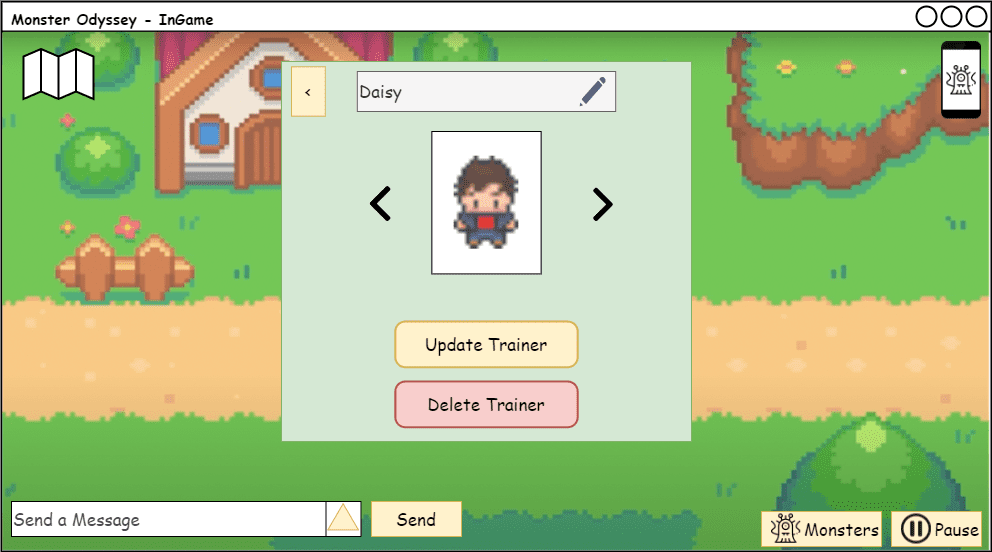
\includegraphics[width=\textwidth]{images/mockups/Bonusfeatures/TrainerSettings/TrainerSetting.png}
        \caption{Trainereinstellungen}
        \label{fig: Trainereinstellungen}
    \end{subfigure}
    \hfill
    \begin{subfigure}[b]{0.4\textwidth}
        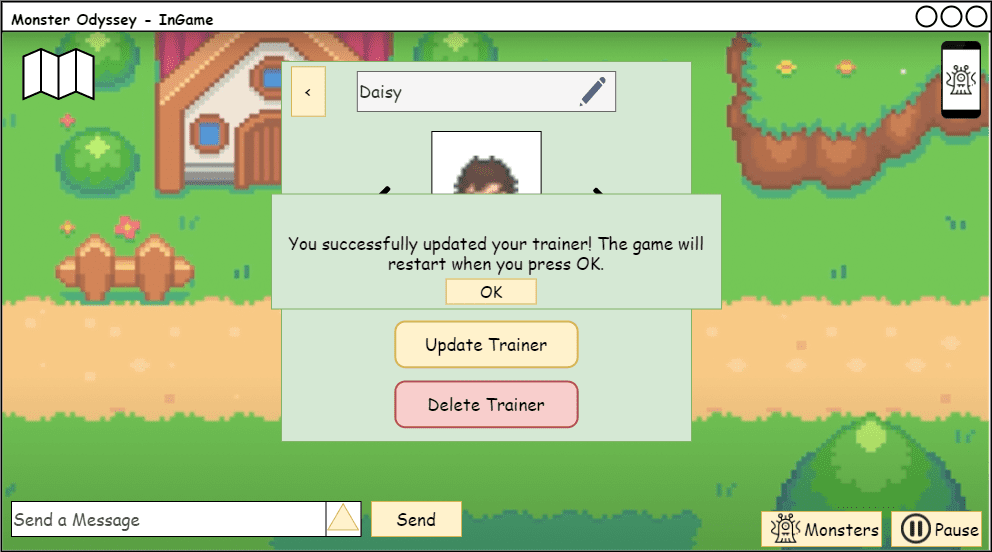
\includegraphics[width=\textwidth]{images/mockups/Bonusfeatures/TrainerSettings/TrainerSettingChanged.png}
        \caption{Trainer aktualisiert}
        \label{fig: Trainer aktualisiert}
    \end{subfigure}
    \caption{Mockup: Aktualisieren des Trainers}
    \label{fig: Aktualisieren des Trainers}
\end{figure}
\begin{figure}[H]
    \centering
    \begin{subfigure}[b]{0.4\textwidth}
        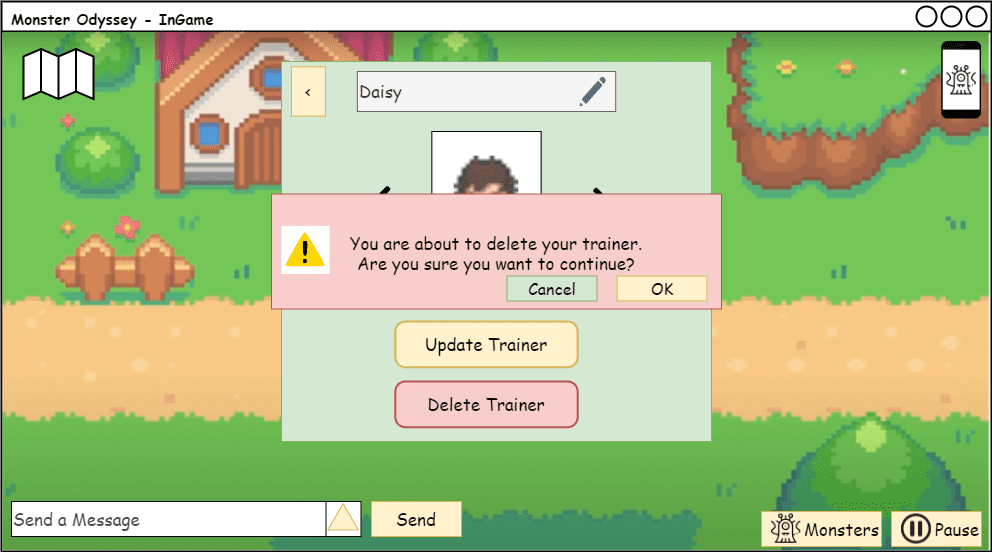
\includegraphics[width=\textwidth]{images/mockups/Bonusfeatures/TrainerSettings/IngameDeleteTrainerPopup.png}
        \caption{Popup für Löschen des Trainers}
        \label{fig: Popup beim Löschen des Trainers}
    \end{subfigure}
    \hfill
    \begin{subfigure}[b]{0.4\textwidth}
        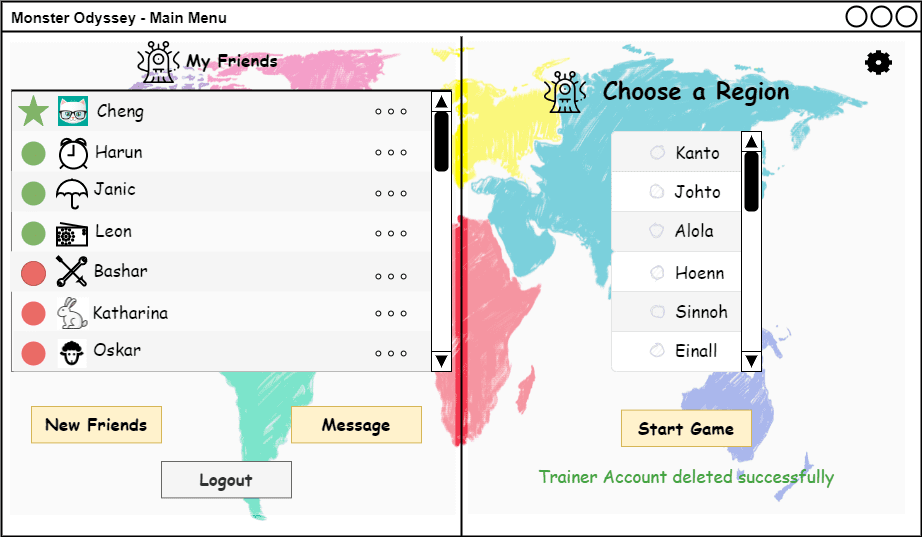
\includegraphics[width=\textwidth]{images/mockups/Bonusfeatures/TrainerSettings/TrainerAccountDeleted.png}
        \caption{Trainer erfolgreich gelöscht}
        \label{fig: Trainer erfolgreich gelöscht}
    \end{subfigure}
    \caption{Mockup: Löschen des Trainers}
    \label{fig: Löschen des Trainers}
\end{figure}
\subsection{Vergleich zwischen Mockups und Implementierung}\label{subsec:vergleich-zwischen-mockups-und-implementierung-trainer-settings}
Die Mockups sind mit der Implementierung übereinstimmend, bis auf das Mockup in der Abbildung~\ref{fig: Trainer erfolgreich gelöscht}. Dafür ist in der Abbildung~\ref{fig: Mockup: Trainer erfolgreich gelöscht} der Audio-Button in der Abbildung~\ref{fig: Implementierung: Trainer erfolgreich gelöscht} fehlend und der Bestätigungstext für das Löschen des Trainers befindet sich über dem Startknopf des Spiels. Der Bestätigungstext in der Abbildung~\ref{fig: Implementierung: Trainer erfolgreich gelöscht} unterscheidet sich ebenso. Dennoch besitzt der Unterschied keine semantischen Folgen. Somit hat der Text dieselbe Semantik wie in der Abbildung~\ref{fig: Mockup: Trainer erfolgreich gelöscht}. 
\begin{figure}[H]
    \centering
    \begin{subfigure}[b]{0.4\textwidth}
        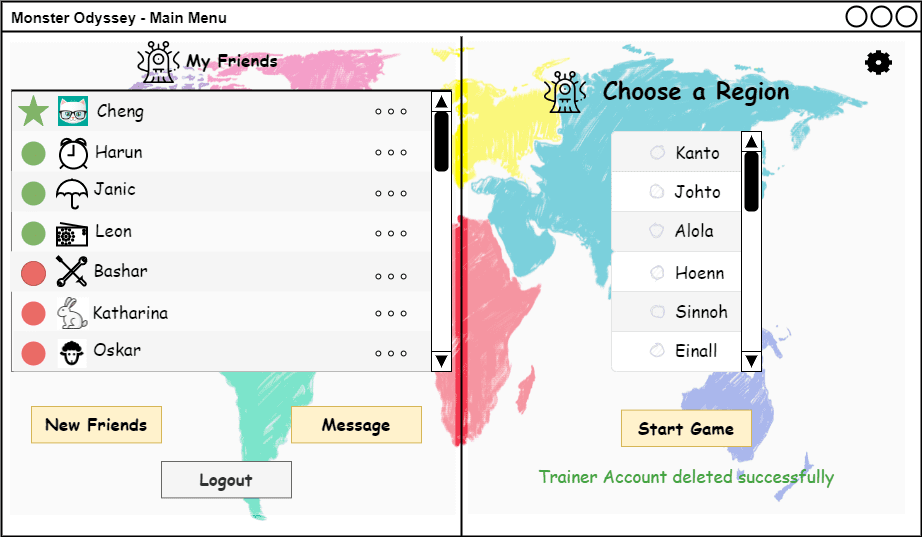
\includegraphics[width=\textwidth]{images/mockups/Bonusfeatures/TrainerSettings/TrainerAccountDeleted.png}
        \caption{Mockup: Trainer erfolgreich gelöscht}
        \label{fig: Mockup: Trainer erfolgreich gelöscht}
    \end{subfigure}
    \hfill
    \begin{subfigure}[b]{0.4\textwidth}
        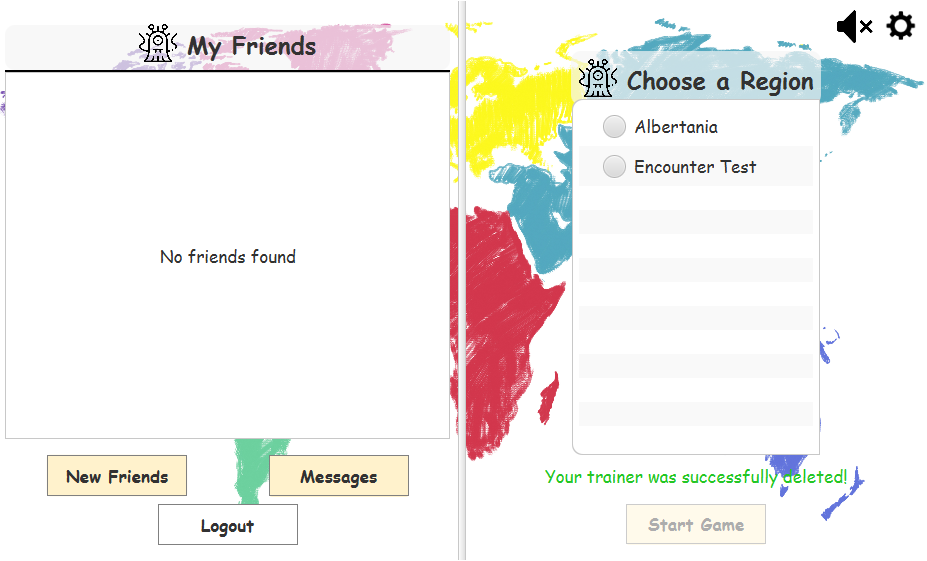
\includegraphics[width=\textwidth]{images/implementation/Bonusfeatures/TrainerSettings/Trainerdeleted.PNG}
        \caption{Implementierung: Trainer erfolgreich gelöscht}
        \label{fig: Implementierung: Trainer erfolgreich gelöscht}
    \end{subfigure}
    \caption{Vergleich: Erweiterung Trainereinstellungen}
    \label{fig: Vergleich: Erweiterung Trainereinstellungen}
\end{figure}
In den Abbildungen~\ref{fig: Vergleich: Trainereinstellungen},~\ref{fig: Vergleich: Trainer aktualisiert} und~\ref{fig: Vergleich: Popup für Löschen des Trainers} ist zu sehen, dass es keine bis geringfügige Unterschiede zwischen den Mockups und der Implementierung gibt, wobei die kleinen Unterscheide keinen Einfluss auf die Funktionalität haben.
\begin{figure}[H]
    \centering
    \begin{subfigure}[b]{0.4\textwidth}
        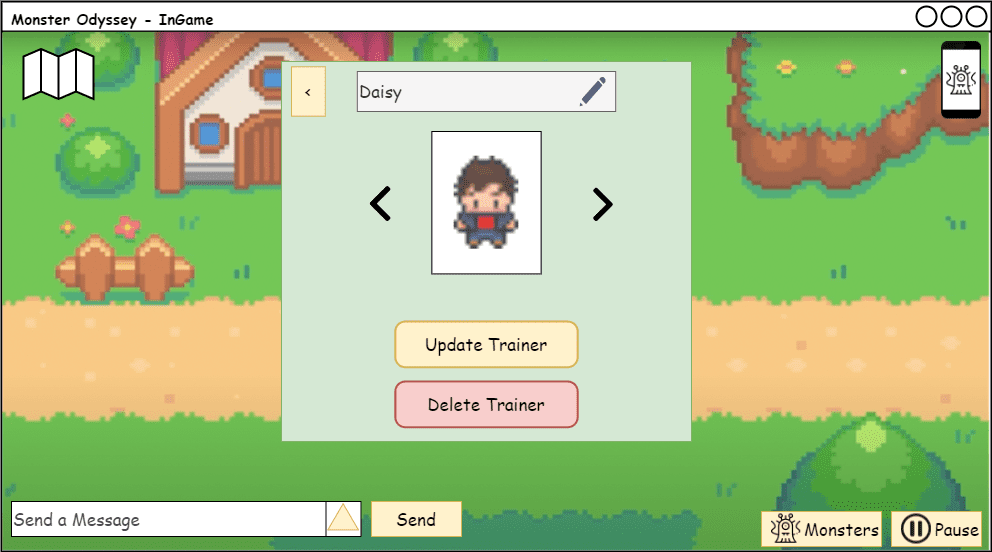
\includegraphics[width=\textwidth]{images/mockups/Bonusfeatures/TrainerSettings/TrainerSetting.png}
        \caption{Mockup: \phantom{Trainer} Trainereinstellungen}
        \label{fig: Mockup: Trainereinstellungen}
    \end{subfigure}
    \hfill
    \begin{subfigure}[b]{0.4\textwidth}
        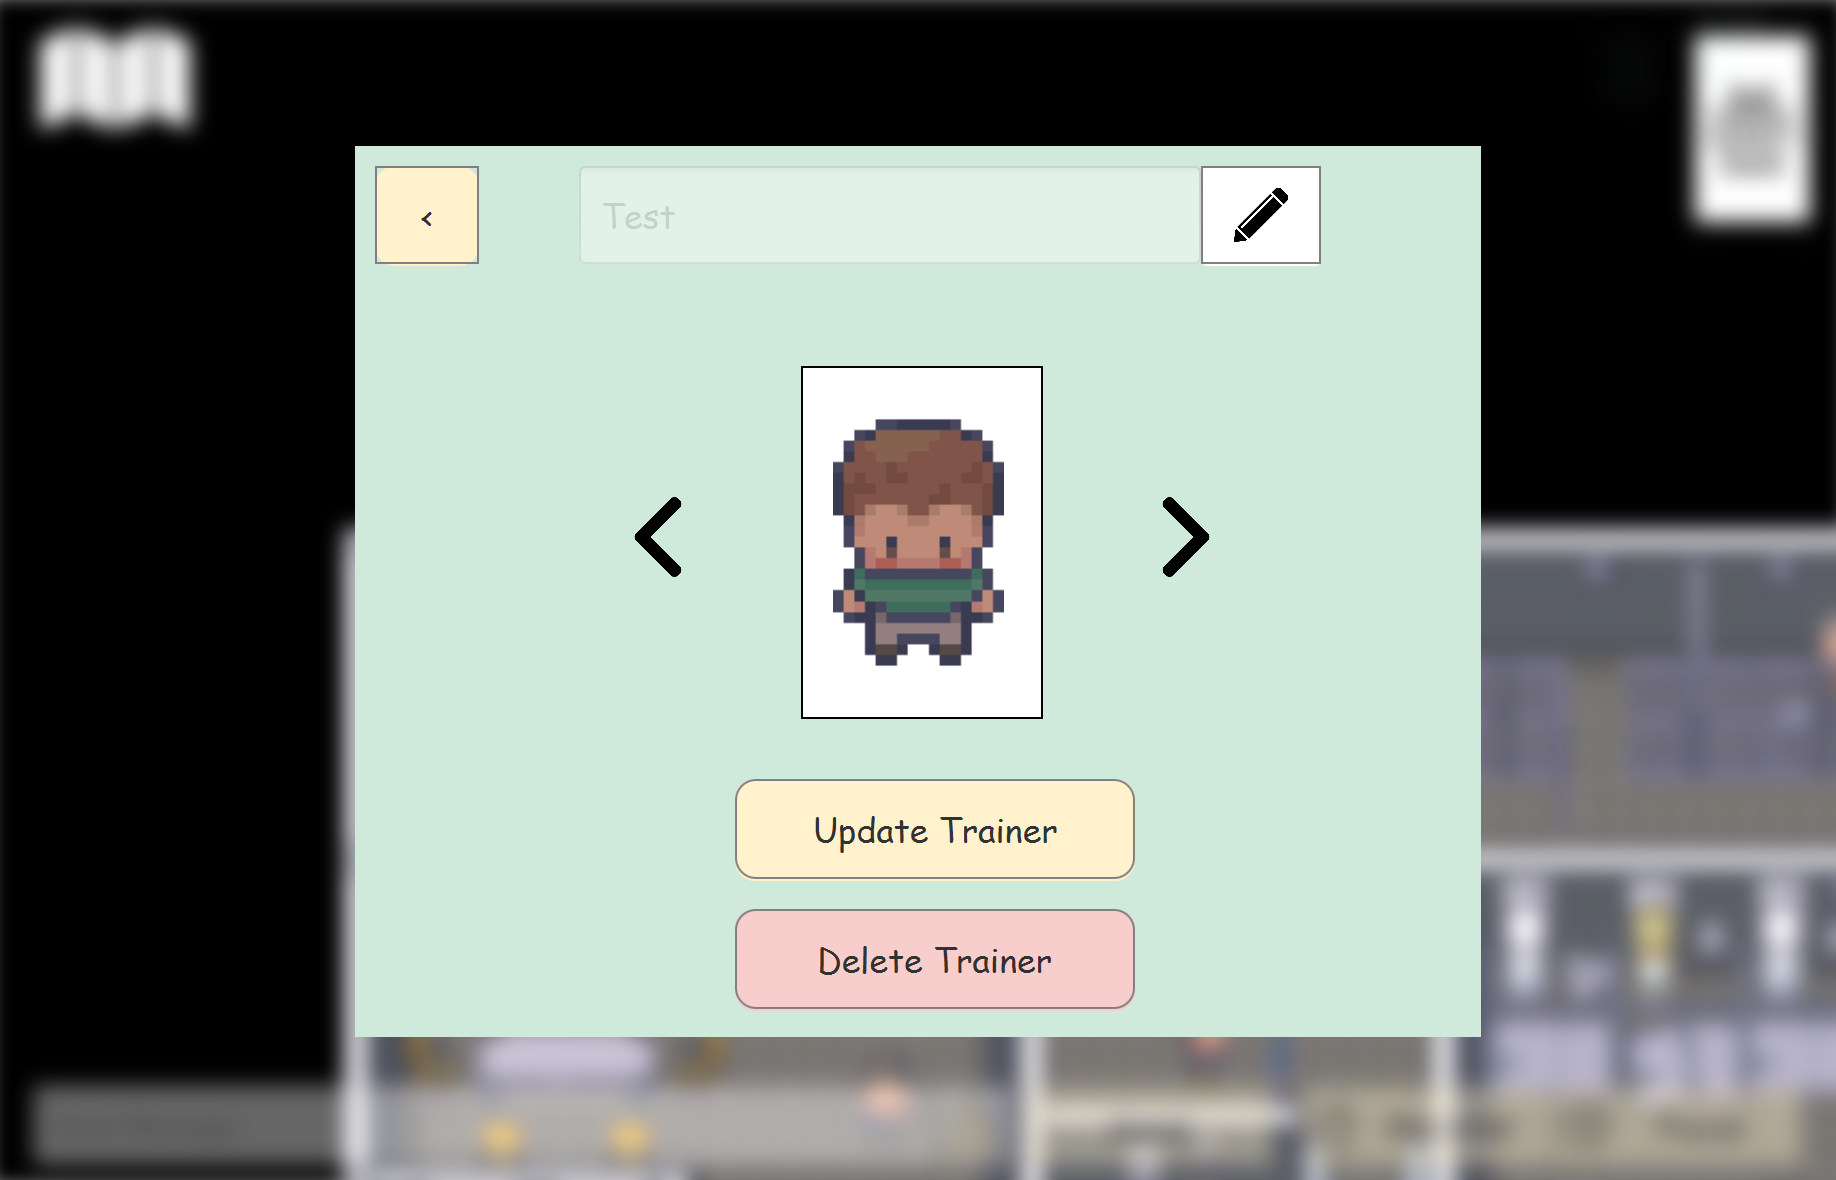
\includegraphics[width=\textwidth]{images/implementation/Bonusfeatures/TrainerSettings/TrainerSettings.png}
        \caption{Implementierung: Trainereinstellungen}
        \label{fig: Implementierung: Trainereinstellungen}
    \end{subfigure}
    \caption{Vergleich: Trainereinstellungen}
    \label{fig: Vergleich: Trainereinstellungen}
\end{figure}
\begin{figure}[H]
    \centering
    \begin{subfigure}[b]{0.4\textwidth}
        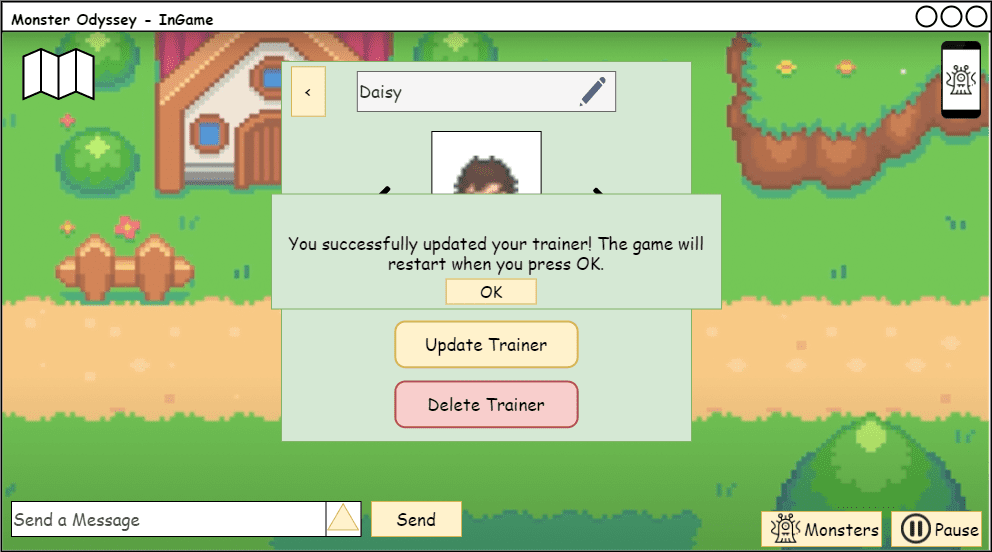
\includegraphics[width=\textwidth]{images/mockups/Bonusfeatures/TrainerSettings/TrainerSettingChanged.png}
        \caption{Mockup: \phantom{Trainer} Trainer aktualisiert}
        \label{fig: Mockup: Trainer aktualisiert}
    \end{subfigure}
    \hfill
    \begin{subfigure}[b]{0.4\textwidth}
        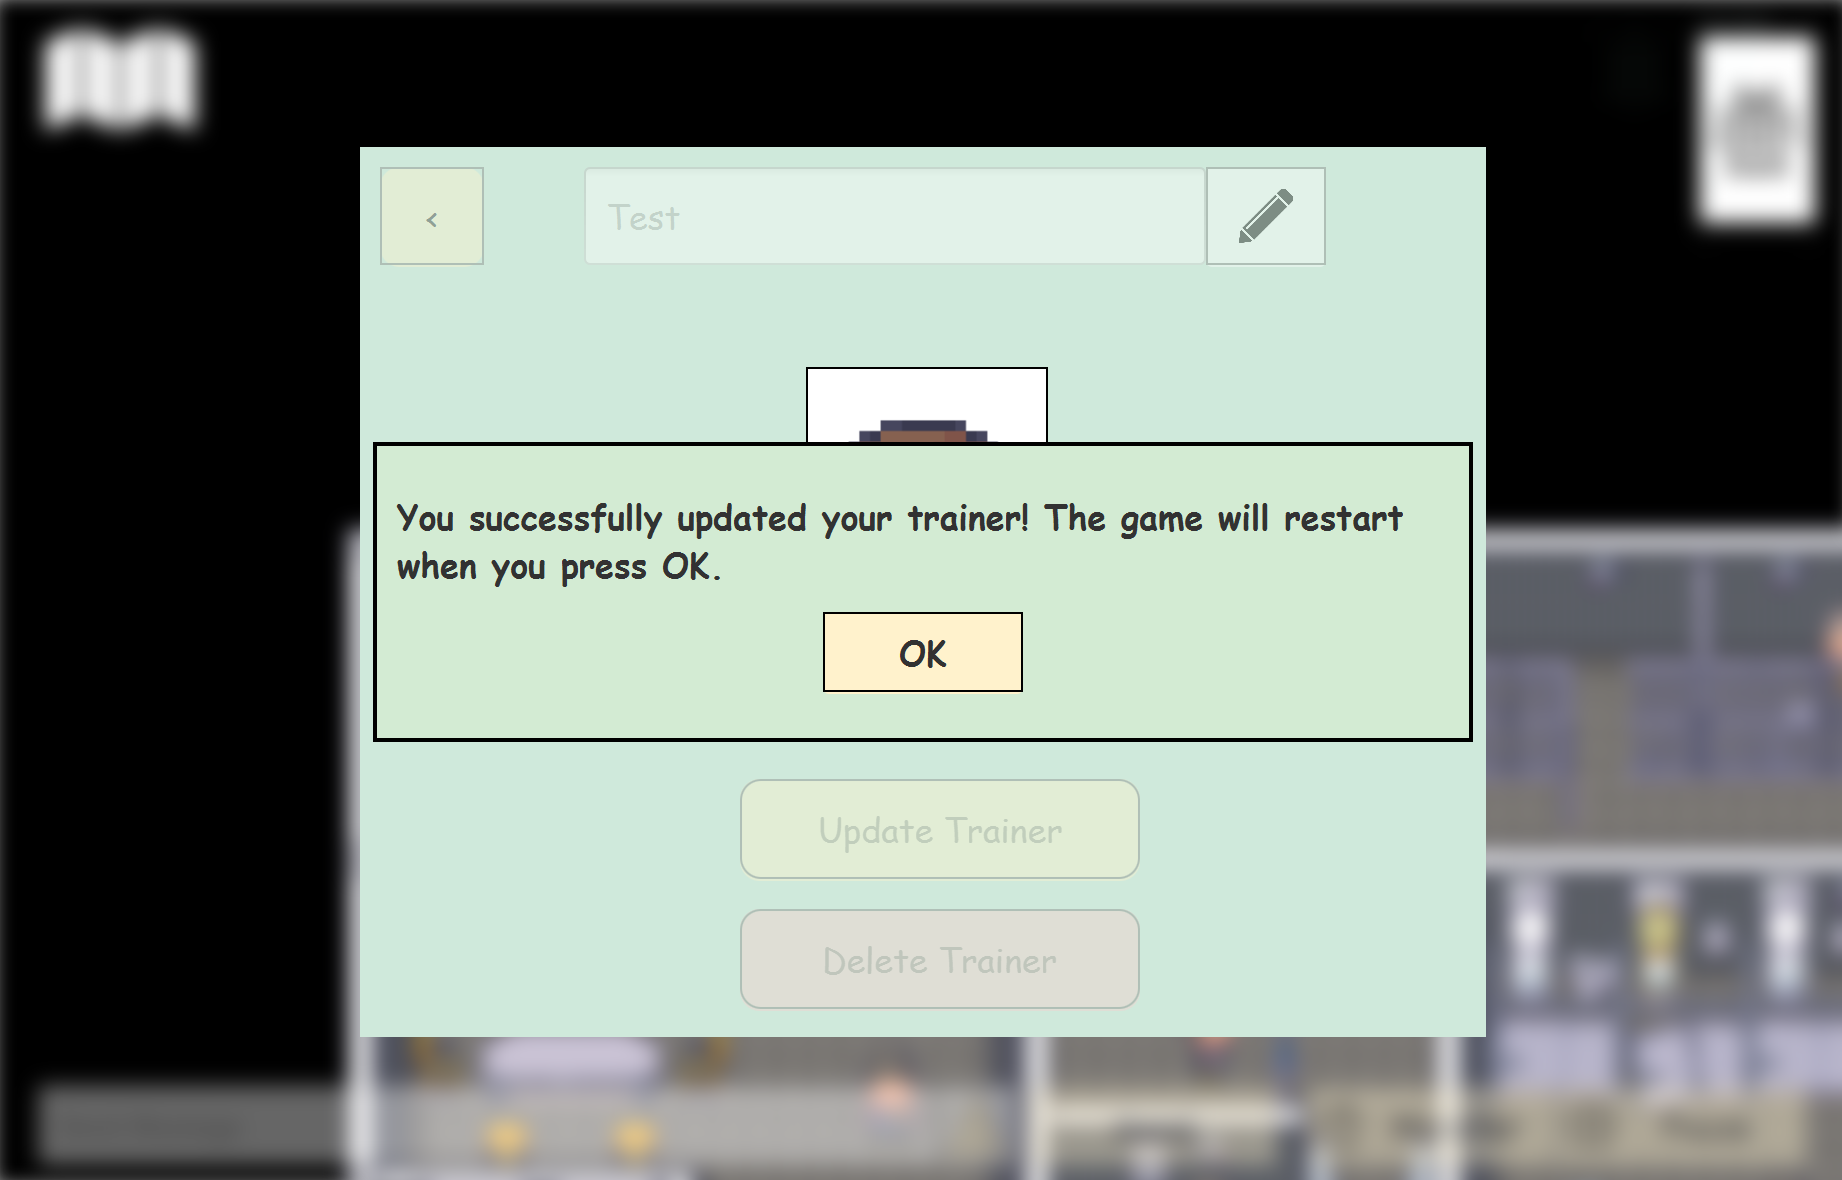
\includegraphics[width=\textwidth]{images/implementation/Bonusfeatures/TrainerSettings/UpdateTrainer.png}
        \caption{Implementierung: Trainer aktualisiert}
        \label{fig: Implementierung: Trainer aktualisiert}
    \end{subfigure}
    \caption{Vergleich: Trainer aktualisiert}
    \label{fig: Vergleich: Trainer aktualisiert}
\end{figure}
\begin{figure}[H]
    \centering
    \begin{subfigure}[b]{0.4\textwidth}
        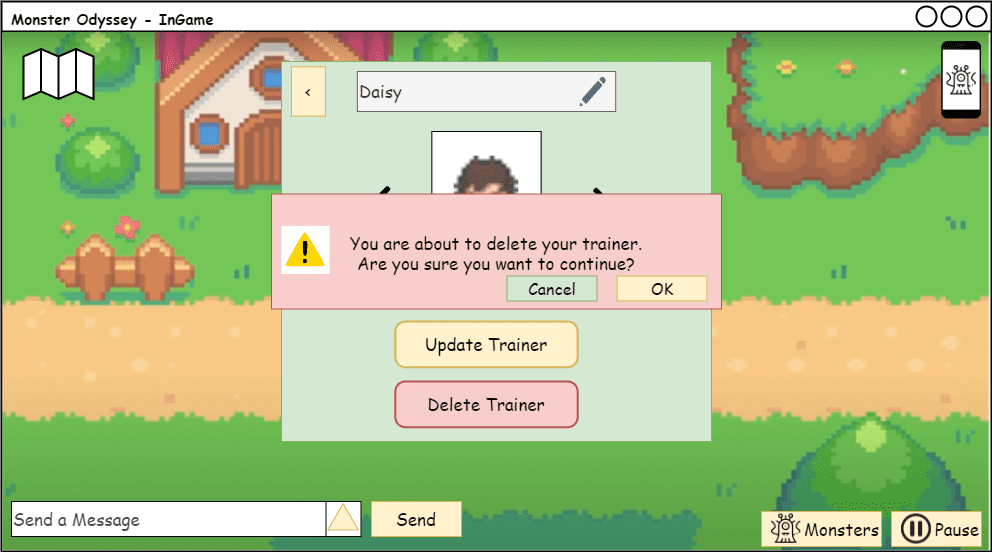
\includegraphics[width=\textwidth]{images/mockups/Bonusfeatures/TrainerSettings/IngameDeleteTrainerPopup.png}
        \caption{Mockup: Popup für Löschen des Trainers}
        \label{fig: Mockup: Popup beim Löschen des Trainers}
    \end{subfigure}
    \hfill
    \begin{subfigure}[b]{0.4\textwidth}
        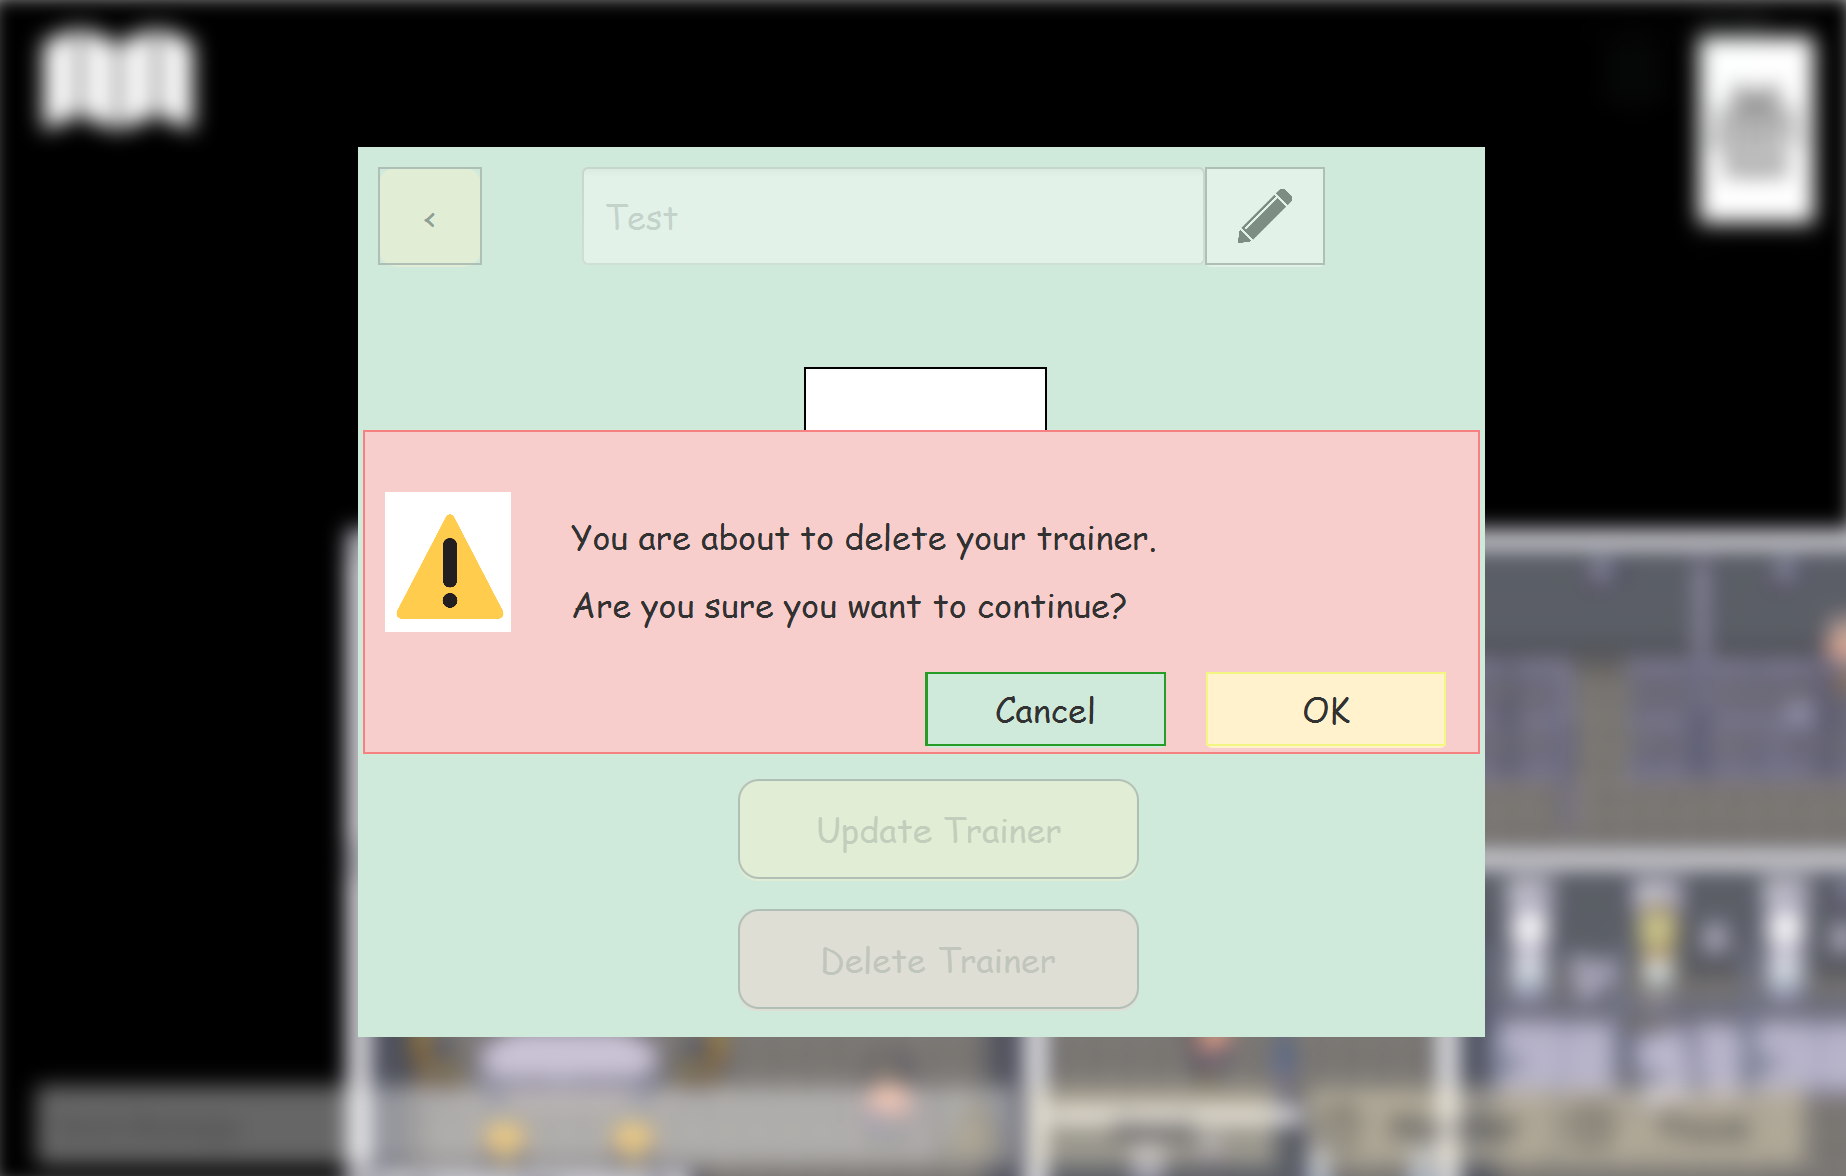
\includegraphics[width=\textwidth]{images/implementation/Bonusfeatures/TrainerSettings/DeleteTrainer.png}
        \caption{Implementierung: Popup für Löschen des Trainers}
        \label{fig: Implementierung: Popup für Löschen des Trainers}
    \end{subfigure}
    \caption{Vergleich: Popup für Löschen des Trainers}
    \label{fig: Vergleich: Popup für Löschen des Trainers}
\end{figure}